\begin{frame}{Markov Decision Processes}
	\begin{block}{Reinforcement Learning}
		General class of algorithms that allow an agent to learn how to behave
		in a stochastic and possibly unknown environment by trial-and-error.
	\end{block}
	
	\begin{block}{Markov Decision Process (MDP)}
		stochastic dynamical system specified by $<\S, \A, \calP, \calR, \gamma>$
		\begin{enumerate}
			\item $(\S, \calS)$ is a measurable state space
			\item $(\A, \calA)$ is a measurable action space
			\item $\calP: \S \times \A \times \calS \to \R$ is a Markov transition kernel
			\item $\calR: \S \times \A \to \R$ is a reward function
			\item $0 < \gamma < 1$ is the discount factor.
		\end{enumerate}
	\end{block}
\end{frame}


\begin{frame}{Policy Gradient Theorem: Statement and Proof}

	\begin{block}{Policy Gradient Theorem}
	Let $\pi_\theta$ be a differentiable policy. For the gradient of the average reward is 
	\begin{equation*}
		\nabla_\theta \rho(\theta) =
		\E[\substack{S \sim d^\theta\\A \sim \pi_\theta}]{\nabla_\theta\log
		\pi_\theta(S,A) Q_{\theta}(S, A)}
	\end{equation*}
	where $d^\theta$ is the stationary distribution of the Markov chain induced by $\pi_\theta$. 
	\end{block}
	\textbf{Proof}\\
	\scalebox{0.8}{%
	$\nabla_\theta V_\theta(s) = \nabla_\theta \int_{\A} \pi_\theta(s,a) Q_\theta(s,a) da = \int_{\A} \left[ \nabla_\theta \pi_\theta(s,a) Q_\theta(s,a) + \pi_\theta(s,a) \nabla_\theta Q_\theta(s,a)\right] da$
	} 
	\scalebox{0.8}{%
	$\nabla_\theta Q_\theta(s,a) = \nabla_\theta \left[ \calR(s,a) - \rho_\theta + \int_{\S} \calP(s,a,s') V_\theta(s') ds' \right] = -\nabla_\theta \rho_\theta + \int_{\S} \calP(s,a,s') \nabla_\theta V_\theta(s') ds'$
		} 
		\scalebox{0.8}{%
	$\nabla_\theta V_\theta(s) = \int_{\A} \nabla_\theta \pi_\theta(s,a) Q_\theta(s,a) da - \nabla_\theta \rho_\theta + \int_\A \pi_\theta(s,a) \int_{\S} \calP(s,a,s') \nabla_\theta V_\theta(s') ds'$
		} 
		\scalebox{0.8}{%
	$\int_{\S} d^\theta(s) \int_{\A} \pi(s,a) \int_{\S} \calP(s,a,s') \nabla_\theta V(s') ds' da ds = \int_{\S} d^\theta(s) \nabla_\theta V_\theta(s) ds$
		} 
		\scalebox{0.8}{%
	$\nabla_\theta \rho_\theta = \int_{\S} d^\theta(s) \int_{\A} \nabla_\theta \pi_\theta(s,a) Q_\theta(s,a) da ds = \int_{\S} d^\theta(s) \int_{\A} \pi_\theta(s,a) \nabla_\theta \log\pi_\theta(s,a) Q_\theta(s,a) da ds$
	}
\end{frame}



\begin{frame}{Monte-Carlo Policy Gradient: Pseudocode}
	\begin{algorithmic}[1]
		\Require Stochastic policy $\pi_\theta$, Initial parameters $\theta_0$, learning rate $\{\alpha_k\}$
		\Ensure Approximation of the optimal policy $\pi_{\theta^*} \approx \pi_*$
		\Repeat
			\State Sample $M$ trajectories $h^{(m)} = \{(s_t^{(m)}, a_t^{(m)}, r_{t+1}^{(m)})\}_{t = 0}^{T^{(m)}}$ under policy $\pi_{\theta_k}$   
			\State Approximate policy gradient 
			\begin{equation*}
				\nabla_\theta J(\theta_k) \approx \frac{1}{M} \sum_{m=0}^M
				 \sum_{u=0}^{T^{(m)}-1} \nabla_\theta\log \pi_{\theta_k} \left(s_u^{(m)}, a_u^{(m)}\right) 
				 \sum_{v \geq u}^{T^{(m)}-1} \gamma^{v-u} r_{v+1}^{(m)}   
			\end{equation*}
			\State Update parameters using gradient ascent $\theta_{k+1} = \theta_k + \alpha_k \nabla_\theta J(\theta_k)$
			\State $k \leftarrow k + 1$
		\Until{converged}
	\end{algorithmic}
\end{frame}


\begin{frame}{Episodic PGPE Algorithm: Pseudocode}
	\begin{algorithmic}[1]
		\Require Controller $F_\theta$, hyper-distribution $p_\xi$, initial guess $\xi_0$, learning rate $\{\alpha_k\}$
		\Ensure Approximation of the optimal policy $F_{\xi^*} \approx \pi_*$
		\Repeat
			\For {$m = 1, \ldots, M$}
				\State Sample controller parameters $\theta^{(m)} \sim p_{\xi_k}$ 
				\State Sample trajectory $h^{(m)} = \{(s_t^{(m)}, a_t^{(m)}, r_{t+1}^{(m)})\}_{t = 0}^{T^{(m)}}$ under policy $F_{\theta^{(m)}}$
			\EndFor
			\State Approximate policy gradient 
		  		\begin{equation*}
		  		\nabla_\xi J(\xi_k) \approx \frac{1}{M} \sum^{M}_{m=1} \nabla_\xi \log p_\xi\left(\theta^{(m)}\right) \left[G\left(h^{(m)}\right)-b\right] 
		  		\end{equation*}
		  		
			\State Update hyperparameters using gradient ascent $\xi_{k+1} = \xi_k + \alpha_k \nabla_\xi J(\xi_k)$
			\State $k \leftarrow k + 1$
		\Until{converged}
	\end{algorithmic}
\end{frame}

\begin{frame}{Natural PGPE Algorithm: Pseudocode}
	\begin{algorithmic}[1]
		\Require Controller $F_\theta$, hyper-distribution $p_\xi$, initial guess $\xi_0$, learning rate $\{\alpha_k\}$
		\Ensure Approximation of the optimal policy $F_{\xi^*} \approx \pi_*$
		\Repeat
			\State Observe current state $s_k$
			\State Draw $\zeta_k \sim \calN(0, I_n)$
			\State Compute controller parameters $\theta_k = \mu_k + \Gamma^T \zeta_k$
			\State Perform action $a_k = F_{\theta_k}(s_k)$ and receive reward $r_{k+1}$
			\State Update average reward estimate $\widehat{\rho}_{k+1} = \widehat{\rho}_{k} + \alpha_k (r_{k+1} - \widehat{\rho}_{k})$
			\State Compute natural policy gradients
				\begin{equation*}
					\begin{split}
						\widetilde{\nabla}_\mu \log p_{\xi_k}(\theta_k) = \theta_k - \mu_k \;\;\;\;\;
						\widetilde{\nabla}_\Gamma \log p_{\xi_k}(\theta_k) = \left(\triu(\zeta_k \zeta_k^T) - \frac{1}{2} \diag(\zeta_k \zeta_k^T) - \frac{1}{2} I \right) \Gamma
					\end{split}
				\end{equation*}
			\State Update eligibility trace $e_{k} = \lambda e_{k-1} + \nabla_\xi \log p_{\xi_k}(\theta_k)$
			\State Update hyper-parameters $\xi_{k+1} = \xi_k + \alpha_k (r_{k+1} - \widehat{\rho}_{k}) e_k$
			\State $k \leftarrow k + 1$
		\Until{converged}
	\end{algorithmic}
\end{frame}



\begin{frame}{Experiment on Synthetic Asset}
	The synthetic asset price is given by
	\begin{equation*}
		Z_t = \exp\left(\frac{z_t}{\max_t z_t - \min_t z_t}\right)
	\end{equation*}
	where $\{z_t\}$ is a random walk with autoregressive trend $\{\beta_t\}$
		\begin{equation*}
			\begin{split}
				z_t &= z_{t-1} + \beta_{t-1} + \kappa \epsilon_t\\
				\beta_t &= \alpha \beta_{t-1} + \nu_t\\
			\end{split}
		\end{equation*}
	The policy used for the PGPE and the NPGPE algorithms is 
	\begin{equation*}
		F_\theta(s) = \sign(\theta \cdot s)
	\end{equation*}
	where
	\begin{equation*}
		\theta \sim \calN(\mu, \diag(\sigma))
	\end{equation*}  
\end{frame}

\begin{frame}[c]{PyBrain's Architecture for a RL Problem}
\begin{figure}[t!]
	\centering
	\begin{tikzpicture}[node distance = 6em, auto, thick]
		\node (rect) at (0,0) [draw,thick,minimum width=8cm,minimum height=6cm] (Experiment) {};
		\node (rect) at (0,1.4) [draw,thick,minimum width=6cm,minimum height=2cm] (Task) {};
		\node (rect) at (0,1.4) [draw,thick,minimum width=3cm,minimum height=1cm] (Environment) {\texttt{Environment}};
		\node (rect) at (0,-1.4) [draw,thick,minimum width=6cm,minimum height=2cm] (Agent) {};
		\node (rect) at (-1.9,-1.4) [draw,thick,minimum width=1.6cm,minimum height=1cm] (Critic) {\texttt{Critic}};
		\node (rect) at (1.9,-1.4) [draw,thick,minimum width=1.6cm,minimum height=1cm] (Learner) {\texttt{Learner}};
		\node (rect) at (0,-1.4) [draw,thick,minimum width=1.6cm,minimum height=1cm] (Actor) {\texttt{Actor}};
		
		\draw (-2.8,3.3) node {\texttt{Experiment}};
		\draw (-2.4,2.7) node {\texttt{Task}};
		\draw (0.8,0) node {\texttt{Action}};
		\draw (-2.25,1.7) node {\texttt{State}};	
		\draw (2.7,0) node {\texttt{Reward}};
		\draw (-2.4,-2.7) node {\texttt{Agent}};
	
		\path [line] (Task.180) --++ (-0.5cm,0cm) |- node [near start]{\texttt{Observation}} (Agent.180);
		\path [line] (Task.0) --++ (+0.5cm,0cm) |- (Agent.0);
		\draw[line] (Environment.180) -- (Task.180);
		\draw[line] (Agent.90) -- (Task.270); 
	\end{tikzpicture}
\end{figure}	
\end{frame}

\begin{frame}[c]{Agent-Environment Interaction in C++}
	\begin{block}{Adapting PyBrain's Architecture}
		\begin{enumerate}
			\item Defined standard interfaces via pure abstract classes
			\item Achieved modularity via polymorphic composition
		\end{enumerate}
	\end{block}
	
	\begin{figure}[h]
		\centering
		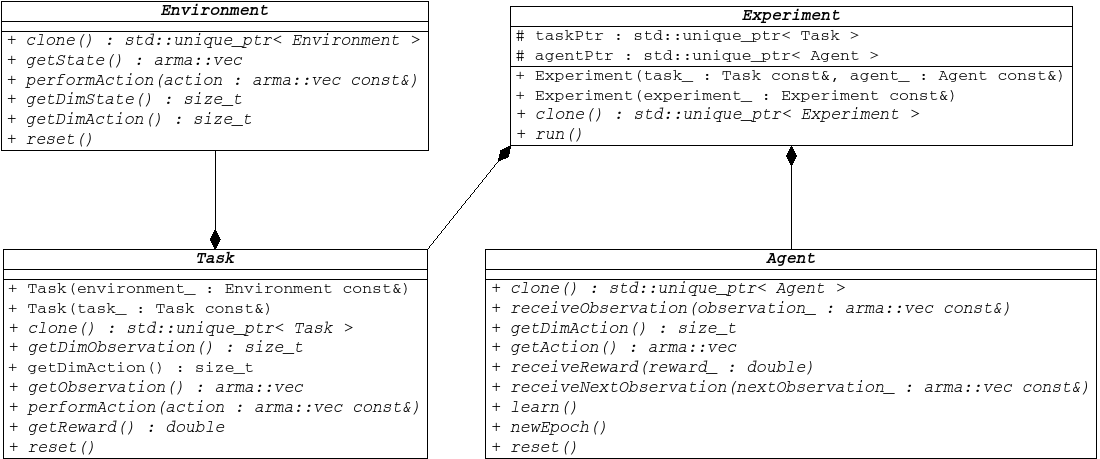
\includegraphics[width=0.8\framewidth]{Images/AgentEnvironmentInteractionReduced}
	\end{figure}
\end{frame}

\begin{frame}[c]{Agent's Architecture in C++}
	\begin{figure}[h]
		\centering
		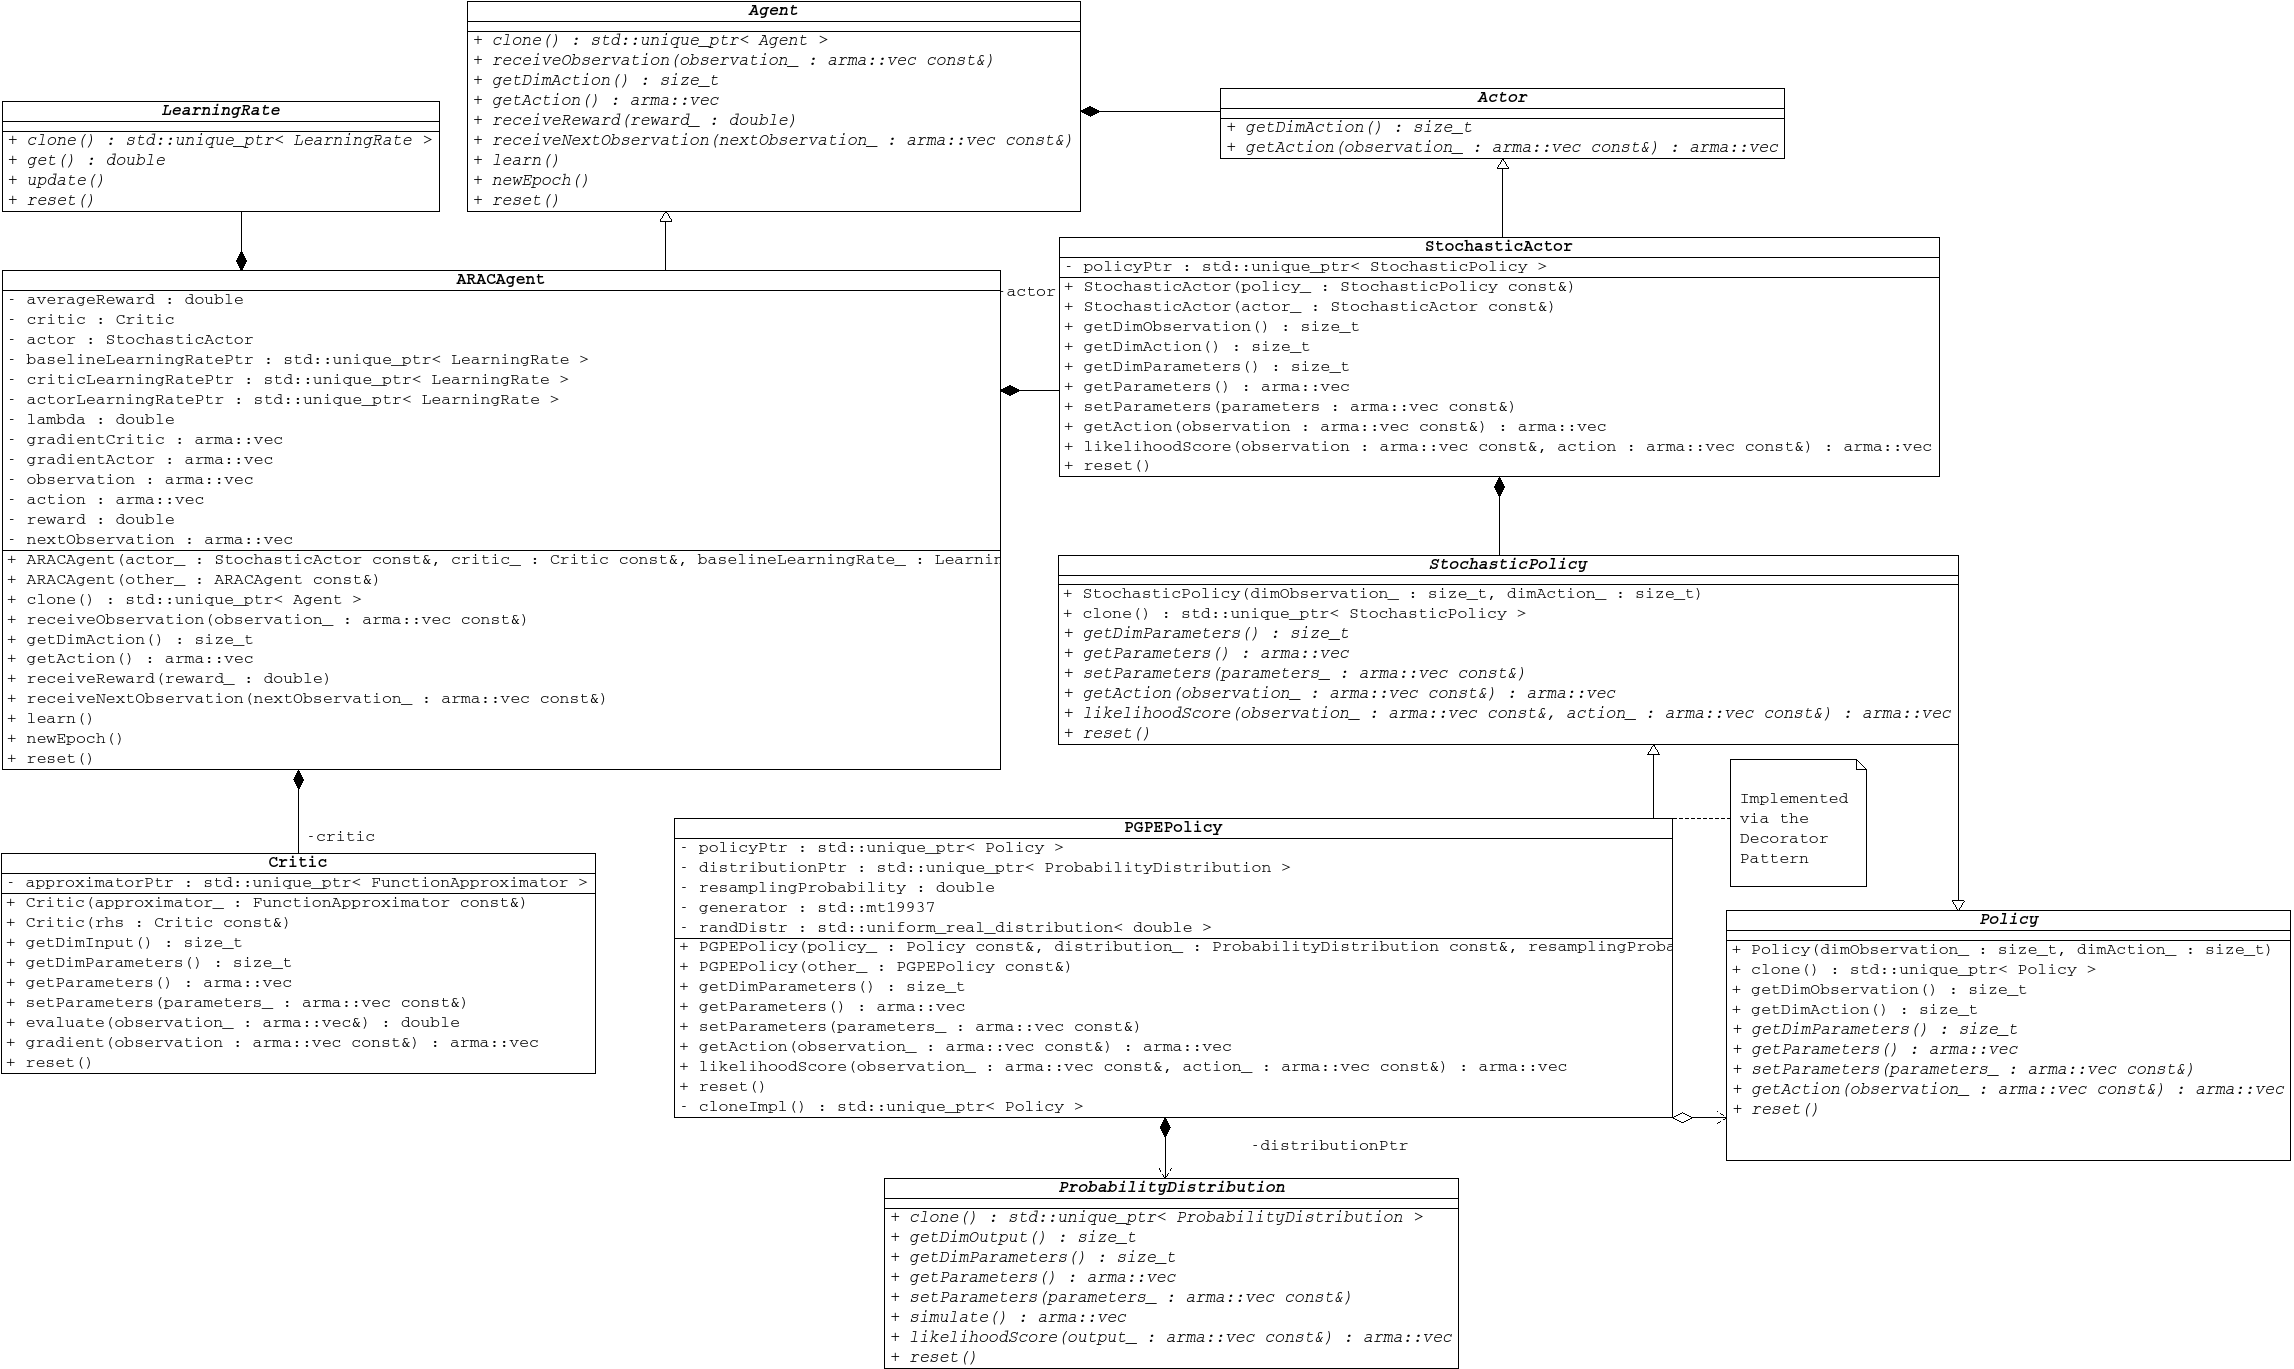
\includegraphics[width=0.8\framewidth]{Images/agent_reduced}
	\end{figure}
\end{frame}

\begin{frame}[c]{Execution Pipeline}
	\begin{block}{\texttt{experiment\_launcher.py}}
		\begin{enumerate}
			\item Program execution is handled by a Python script
			\item Responsible for analyzing the output of the C++ engine
		\end{enumerate}
	\end{block}

	\begin{figure}
		\centering
		\resizebox{0.8\framewidth}{!}{%
		\begin{tikzpicture}[node distance = 6em, auto, thick]
			\node (rect) at (-9.5,-2) [DimGray,draw,thick,minimum width=3cm,minimum height=3cm] (generate_synthetic_series) {};
			\node (rect) at (0,0) [DimGray,draw,thick,minimum width=15cm,minimum height=10cm] (experiment_launcher) {};
			\node (rect) at (+9,-2) [IndianRed,draw,thick,minimum width=2cm,minimum height=3cm] (convergence) {};
			\node (rect) at (+9,+2) [IndianRed,draw,thick,minimum width=2cm,minimum height=3cm] (performance) {};
			\node (rect) at (-6,2) [IndianRed,draw,thick,minimum width=2cm,minimum height=3cm] (input) {};
			\node (rect) at (-6,-2) [IndianRed,draw,thick,minimum width=2cm,minimum height=3cm] (synthetic) {};
			\node (rect) at (-2,0) [SteelBlue, draw,thick,minimum width=4cm,minimum height=8cm] (main_thesis) {};
			\node (rect) at (2,2) [IndianRed,draw,thick,minimum width=2cm,minimum height=3cm] (output) {};
			\node (rect) at (2,-2) [IndianRed,draw,thick,minimum width=2cm,minimum height=3cm] (debug) {};
			\node (rect) at (5.5,0) [DimGray,draw,thick,minimum width=3cm,minimum height=3cm] (postprocessing) {};
			
			\draw (0,5.5) node {\lstinline{experiment_launcher.py}};
			\draw (-9.5,0) node {\lstinline{generate_synthetic_series.py}};
			\draw (-6,-4) node {\lstinline{synthetic.csv}};
			\draw (-7.8,4) node {\lstinline{Single_Synth_RN_P0_F0_S0_N5.pot}};	
			\draw (5.5,2) node {\lstinline{postprocessing.py}};
			\draw (2,4) node {\lstinline{output.csv}};
			\draw (2,-4) node {\lstinline{debug.csv}};
			\draw (9.5,4) node {\lstinline{performance.csv}};
			\draw (9.5,-4) node {\lstinline{convergence.csv}};
			\draw (-2,0) node {\lstinline{main_thesis}};	
		
			\draw[line] (generate_synthetic_series.0) -- (synthetic.180);
			\draw[line] (debug.0) -- (postprocessing.180);
			\draw[line] (output.0) -- (postprocessing.180);
			\draw[line] (postprocessing.0) -- (performance.180);
			\draw[line] (postprocessing.0) -- (convergence.180);
			\draw[line] (input.0) -- (main_thesis.135);
			\draw[line] (synthetic.0) -- (main_thesis.225);
			\draw[line] (main_thesis.45) -- (output.180);
			\draw[line] (main_thesis.315) -- (debug.180);
		\end{tikzpicture}}
	\end{figure}
\end{frame}